\documentclass{beamer}
\usepackage{style}

\title{Evaluation of the Dash shared memory supercomputer}
\author{Hallgeir Lien}
\date{May 2, 2011}
\begin{document}

\maketitle

\begin{frame}
\frametitle{Dash Specifications}
\begin{itemize}
\item 64 compute nodes total
\pause
\item Each node has two Intel Xeon E5530 2.4GHz Nehelem quad core CPUs
\pause
\item 512 compute cores, 4.9 TFLOPS
\pause
\item 48GB of main memory per node, plus 4TB of shared flash storage
\pause
\end{itemize}
\end{frame}

\begin{frame}
\frametitle{Shared Memory Supercomputer}
Dash has a virtual shared memory multiprocessing system, vSMP
\begin{itemize}
\item Developed by ScaleMP
\pause
\item Aggregates cores and memory across 16 compute nodes
\pause
\item Memory of all nodes accessible through a unified address space
\pause
\item Parallellization possible using OpenMP and pthreads. Convenient!
\end{itemize}
\end{frame}

\begin{frame}
\frametitle{vSMP specifics}
\begin{itemize}
\item Memory pages are cached locally on each node
\pause
\item Large page sizes: 4KB
\pause
\item Has cache coherency
\pause
\item Writing to pages causes invalidation
    \begin{itemize}
        \item Frequently reading frequently updated pages is expensive
        \pause
        \item We would want to cleverly partition and pad the data
    \end{itemize}
\pause
\item Ownership of data is determined on a first-write policy
\end{itemize}
\end{frame}

\begin{frame}
\frametitle{Test application: Aliev-Panfilov}
The Aliev-Panfilov model models excitation in heart cells.
\pause
\begin{itemize}
\item 5-point 2D stencil
\pause
\item Simple communication with neighboring processors; border of ghost cells, one element wide on all sides
\pause
\item Also has an ODE part
\pause
\item FLOPS per element: 27 (7 for PDE, 20 for ODE)
\end{itemize}
\end{frame}

\begin{frame}
\frametitle{Results from Triton}
I have previously run this application on Triton with MPI.
\pause
\begin{itemize}
\item Weak scaling baseline: $512\times 1024$ elements per core
\begin{itemize}
\item On 512 cores: about 1 GFLOPS/s per core
\pause
\item On 64 cores: about 1.38 GFLOPS/s per core
\end{itemize}
\pause
\item Speedup baseline on fixed problem sizes of $2048^2$: 
\begin{itemize}
    \item On 8 cores (on same node): 4.6x speedup
    \pause
    \item On 32 cores (four nodes): 22x speedup
\end{itemize}
\end{itemize}
\end{frame}

\begin{frame}
\frametitle{First implementation of Aliev-Panfilov on Dash (vSMP)}
\begin{itemize}
\item Pages are large, so we want long, fat partitioning of the data over each core
\end{itemize}
\pause
\begin{figure}
\begin{tabular}{c|c|c|c|>{\columncolor[gray]{.8}}c|c|c|c}
& & & & & & &\\
\hline
& & & & & \cellcolor[rgb]{1,.5,.5}& &\\
\hline
\cellcolor[rgb]{.5,1,.5}& \cellcolor[rgb]{.5,1,.5}& \cellcolor[rgb]{.5,1,.5}& \cellcolor[rgb]{.5,1,.5}&\cellcolor[rgb]{1,.5,.5} & \cellcolor[rgb]{.5,.5,1}& \cellcolor[rgb]{1,.5,.5}&\\
\hline
& & & & & \cellcolor[rgb]{1,.5,.5}& &\\
\hline
& & & & & & &\\
\hline
& & & & & & &\\
\end{tabular}
\end{figure}
Figure: Gray is ghost cells. All green cells are on one page (including the ghost cell on the same row). Processor to the right requires all red cells to compute the blue cell. This is true for all cells in that column.
\pause

This means a lot of wasted bandwidth.
\end{frame}

\begin{frame}
\frametitle{First implementation of Aliev-Panfilov on Dash (vSMP)}
\begin{itemize}
\item Because of this, I used fat partitions spanning the whole matrix.
\pause
\item Doesn't scale well (but not that important for as few as 128 cores).
\pause
\item I padded and aligned each row so that $E[i]\mod 4096/8 = 0$ for all rows $i$, that is, each row starts at a page boundary
\pause
\item This prevents pages spanning over more than one row, which would lead to false sharing
\end{itemize}
\end{frame}

\begin{frame}
\frametitle{First results - OpenMP}
\begin{figure}
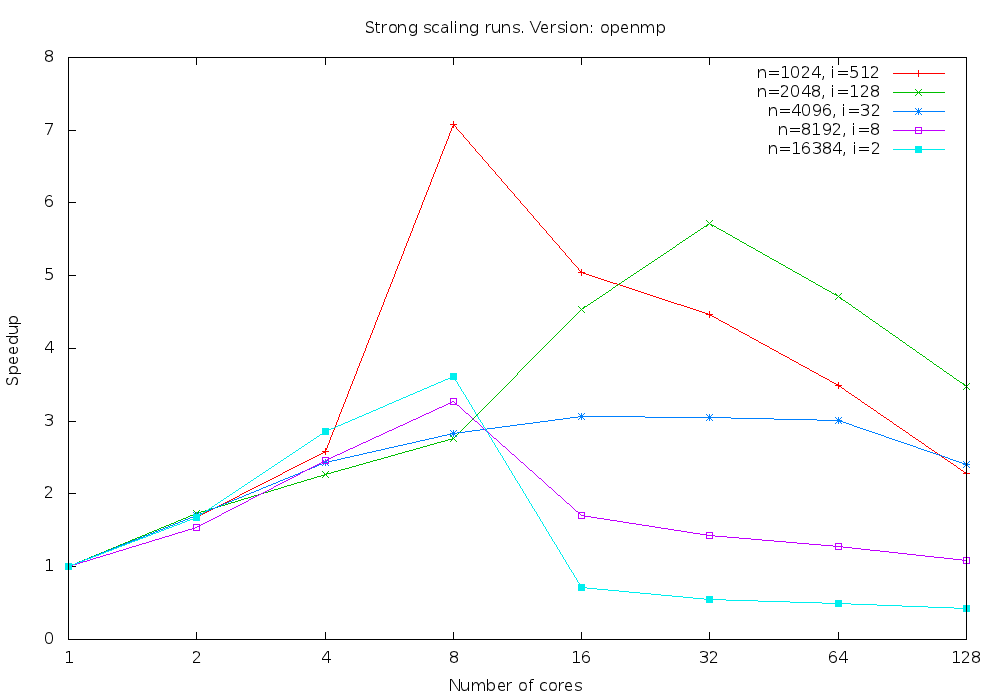
\includegraphics[width=\textwidth]{gfx/padding_strong_scaling_openmp_speedup}
\end{figure}
\end{frame}

\begin{frame}
\frametitle{First results - Pthreads}
\begin{figure}
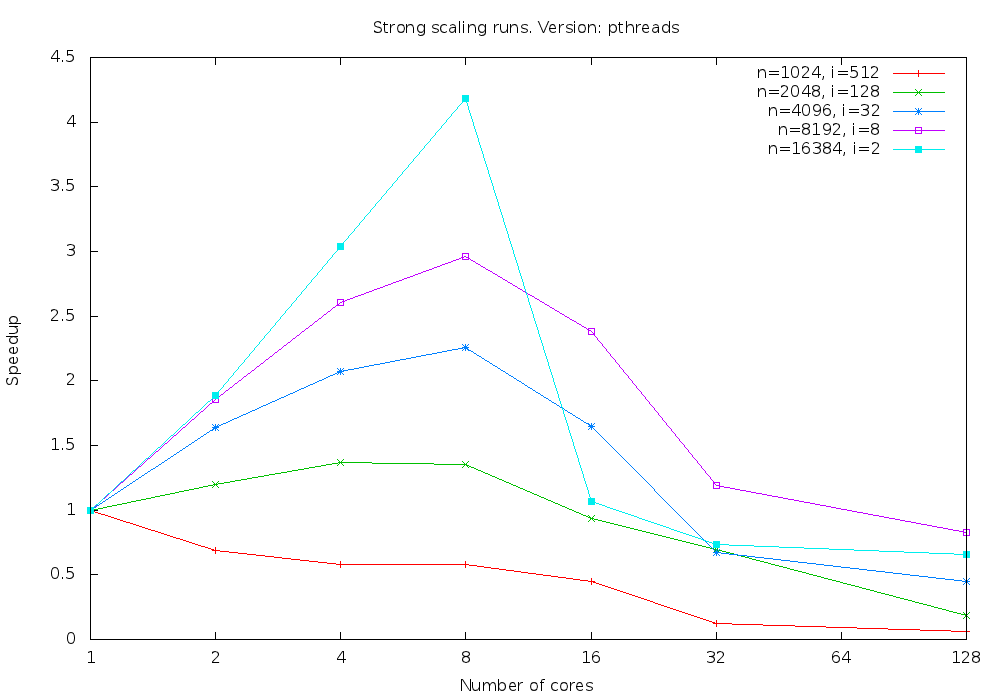
\includegraphics[width=\textwidth]{gfx/padding_strong_scaling_pthreads_speedup}
\end{figure}
\end{frame}

\begin{frame}
\frametitle{First results}
Both implementations show the same trend.
\pause
\begin{itemize}
\item Once we go beyond one node, performance drops considerably.
\pause
\item Only exception: Mid-sized problems ($n=2048$ and $n=4096$) for OpenMP (though still horrible performance; 0.07 GFLOPS/s per core)
\item What's happening?
\end{itemize}

Possible explainations: Mid-sized problems are large enough to speed up slightly without causing too much communication overhead.
\pause
$1024^2$ is too small; communication is too expensive (?)
\end{frame}

\begin{frame}
\frametitle{Second attempt}
I partitioned the data into separate partitions with multiple malloc()s.
\pause
I let each processor initialize its own partition. This should cause that processor to "own" the data.
\pause
More explicit data motion between processors, so it's easier to see what's going on.
\end{frame}

\begin{frame}
\frametitle{Second attempt}
I partitioned the data into separate partitions with multiple malloc()s.
\pause
I let each processor initialize its own partition. This should cause that processor to "own" the data.
\pause
More explicit data motion between processors, so it's easier to see what's going on.
\end{frame}



\end{document}
